\documentclass[11pt, a4paper]{article}
\usepackage[english,spanish, es-tabla]{babel}
\usepackage[top=2.5cm, left=2.5cm, right=2.5cm, bottom=2.5cm]{geometry}
\usepackage{mystyle_2}
\usepackage{mycolours}
\usepackage{mytcolorbox}
\usepackage{mycommands}
\usepackage{microtype}
\usepackage{pdflscape}
\usepackage{rotating}
\usepackage{tabularray}
\UseTblrLibrary{siunitx}

\usepackage[hang,flushmargin]{footmisc} % para que en las notas al pie no me pongo sangría en el párrafo.


\usepackage{chemmacros}
\chemsetup[redox]{pos=top,roman=false} %estados de oxidación arábicos y en la parte superior

\DefTblrTemplate{contfoot-text}{normal}{Continúa en la siguiente página}
\SetTblrTemplate{contfoot-text}{normal}
\DefTblrTemplate{conthead-text}{normal}{(Continuación)}
\SetTblrTemplate{conthead-text}{normal}
\usepackage{lastpage} %para indicar el número de páginas totales
\usepackage{fancyhdr}
\setlength{\headheight}{43.00pt}
\pagestyle{fancy}
\fancyhf{}
\chead{}
\rhead{Dpto. Física y Química}
\lhead{Formulación Inorgánica}
\cfoot{Página \thepage\ de \pageref{LastPage}}

\titleformat{\section}
    {\normalfont\Large\sffamily\bfseries\color{darkblue}}
    {\tcbox[colback=darkblue, colframe=darkblue, coltext=blue!1, on line, boxsep=0pt, left=4pt, right=4pt, top=4pt, bottom=4pt]{\thesection}}{0.5em}{}


\titleformat{\subsection}
    {\normalfont\large\sffamily\bfseries\color{darkblue!80}}
    {\hspace{2mm}\tcbox[colback=darkblue!70, colframe=darkblue, coltext=blue!1, on line, boxsep=0pt, left=4pt, right=4pt, top=4pt, bottom=4pt]{\thesubsection}}{0.5em}{}

\begin{document}
\begin{titlepage}
    \vspace*{5cm}
    \begin{center}
        {\Huge{ \bfseries Nomenclatura Inorgánica}}
    \end{center}
    \vspace*{2cm}
    \begin{center}
        {\huge  IUPAC 2005}
    \end{center}
    \vspace*{5cm}
    \begin{center}
        {\Large IES José Conde García (Almansa)}
    \end{center}
    
    
    %{\Large \bfseries IES Escultor José Luís Sánchez\par}
    %{\Large \bfseries Almansa (Albacete)\par}

\end{titlepage}
\spacing{1.3}
\tableofcontents
\newpage

\section{Introducción}

El orden en el que aparecen los elementos en las fórmulas es importante y deben seguir las siguientes reglas, poniéndose a la derecha los elementos que están más a la derecha del siguiente gráfico:

\begin{figure}[H]
    \centering
    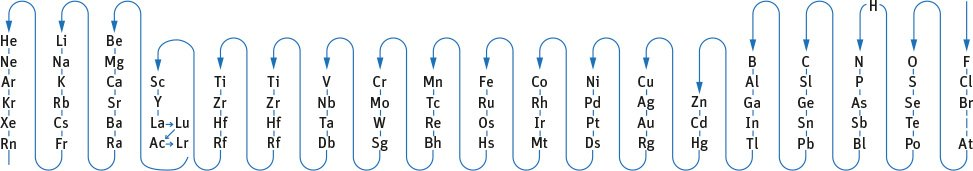
\includegraphics[scale=0.45]{images/orden_elementos.jpg}
\end{figure}

A continuación, se dan una serie de conceptos que es interesante conocer:
\begin{enumerate}[label=\numberballred]
    \item \negrita{Tabla periódica}: disposición de los elementos químicos ordenador por su número atómico creciente en columnas (grupos) y en filas (periodos) presentado de modo que destaquen sus propiedades periódicas.
    \item \negrita{Formulación}: la formulación química consiste en la representación de los elementos que forman parte de un compuesto. Además de la representación se encuentra la proporción de los elementos que intervienen así como el número de átomos que forman la molécula.
    \item \negrita{Fórmula}: combinación de símbolos químicos que expresa la composición de la sustancia.
    \item \textbf{Estado de Oxidación}: también llamado número o grado de oxidación, es un indicador del grado de oxidación es decir ganancia o pérdida de electrones de un átomo o un compuesto. Formalmente puede ser positivo, negativo o cero. Se escriben con número arábicos precedidos del signo \(+1\), $+2$, $0$, $-1$, $-2$ \dots.
    \item \textbf{Valencia}: se define como el número de enlaces que un átomo del elemento forma para unirse con otros átomos. La valencia de un elemento es la capacidad de combinación de un átomo.
\end{enumerate}

\section{Tipos de nomenclatura}
Según la IUPAC, la nomenclatura en química inorgánica la posemos clasificar en tres tipos:
\begin{enumerate}
    \item \textbf{\uline{Nomenclatura sitemática}}. Es aquella que a partir de su nombre y siguiendo unas reglas sistemáticas se puede conocer la composición química. Esta nomenclatura a su vez se puede dividir en tres:
          \begin{enumerate}
              \item \textbf{Adición}. Recoge el nombre de las sustancias químicas en las que a un átomo central se le unen los demás átomos como si fueran ligandos (grupos de átomos que se unen a un átomo central), es útil para nombrar \blueremark{oxocompuestos} y \blueremark{compuestos de coordinación}. Esta nomenclatura considera que un compuesto o una especie es una combinación de un átomo central o átomos centrales con átomos ligados (unidos).
              \item \textbf{Composición}. También recibe el nombre de \textbf{nomenclatura estequiométrica} y está basada en la composición y no en la estructura. Esta nomenclatura da información sobre los átomos y la composición que lo forman mediante el uso de prefijos \blueremark{numerales} (multiplicadores), números o estados de oxidación, o números de carga.
                    \begin{enumerate}[label=\itembolascolor{\arabic*}{blue}]
                        \item \textbf{Usando prefijos multiplicadores} (mono-, di-, tri-, tetra-, penta-, hexa-, etc \dots).
%                              \begin{center}
%                                  \begin{figure}[H]
%                                      \centering
%                                      \SetTblrInner{rowsep=4pt}
%                                      \begin{tblr}{colspec={Q[c,m,1cm] Q[c,m, 3cm] | Q[c,m, 1cm] Q[c,m, 3cm]},
%                                          hline{1,Z} = {1pt},
%                                                  hline{2} = {1pt},
%                                                  hline{3-Y} = {dashed},{0.25pt}
%                                              }
%                                          \SetRow{gray!50} \textcolor{black}{nº} & \textcolor{black}{Prefijo} & \textcolor{black}{nº} & \textcolor{black}{Prefijo}\\
%                                          1 & mono & 6 &    hexa      \\
%                                          2 & di   & 7 &     hepta        \\
%                                          3 &   tri & 8 &     octa  \\
%                                          4 &   tetra & 9 &      nona      \\
%                                          5 &   penta  & 10 &      deca  &     \\
%                                      \end{tblr}
%                                  \end{figure}
%                              \end{center}

                        \item \textbf{Números de oxidación de los elementos} Se indican con  números romanos.
                        \item \textbf{Número de carga de los iones} Se indican con números arábicos.
                    \end{enumerate}
              \item \textbf{Sustitución}. Está basada en la nomenclatura de hidruros no metálicos, que se nombran como hidrocarburos y empleando los sufijos necesarios. La IUPAC acepta los nombres tradicionales como agua (\ch{H2O}) y amoniaco (\ch{NH3})
          \end{enumerate}
    \item \textbf{\uline{Nomenclatura semisitematica}}. Es aquella que aún con reglas sistemáticas, no podemos conocer la composición química.
    \item \textbf{\uline{Nomenclatura tradicional (o vulgar)}}. Se identifica la sustancia sin seguir reglas sistemáticas.
\end{enumerate}


\section{Compuestos binarios}\label{sec:binarios}

\subsection{Compuestos con oxígeno}\label{sec:compuestos_oxigeno}

\subsubsection{Óxidos}\label{sec:oxidos}

Compuestos formados por \blueremark{oxígeno} + un elemento que puede ser un metal o no metal a excepción de los \textbf{halógenos}.
En este tipo de compuestos el oxígeno siempre tiene estado de oxidación \azul{($-2$)} quedando representado como  \ch{O^2-}

\vspace*{8pt}
\xmybox{\bfseries ¿Cómo se formulan?}

\begin{enumerate}[label=\itembolascolor{\arabic*}{green!50!black}]
    \item Escribimos el oxígeno a la derecha.
    \item Escribimos el elemento a la izquierda.
    \item Ponemos encima de cada elemento su correspondiente estado de oxidación.
    \item Intercambiamos los estados de oxidación como subíndices en valor absoluto.
    \item Simplificamos la fórmula si es posible.
\end{enumerate}

\textbf{\uline{Ejemplos:}}

\ballnumber{1} : Óxido de sodio \ch{->} \ox{+1,Na} \ox{-2,O} \ch{->} \ch{Na2O}

\ballnumber{2} : Óxido de calcio \ch{->} \ox{+2,Ca} \ox{-2,O} \ch{->} \ch{Ca2O2} \ch{->} \ch{CaO}

\vspace*{2mm}
\xmybox{\bfseries ¿Cómo se nombran?}

\begin{enumerate}[label=\itembolascolor{\arabic*}{blue}]
    \item \textbf{\uline{Nomenclatura de multiplicadores}}. La nomenclatura sigue las siguientes reglas:
          \begin{center}
              \textcolor{blue}{prefijo\subin{1}} \textcolor{blue}{óxido} + de + \textcolor{red}{prefijo\subin{2}} \textcolor{red}{nombre del elemento}
          \end{center}

          \begin{enumerate}[label=\textcolor{red}{$\bullet$}]
              \item Prefijo\subin{1}: Indica el número de oxígenos.
              \item Prefijo\subin{2}: Indica el número de elementos distintos al oxígeno.
          \end{enumerate}

          El prefijo \blueremark{mono} puede omitirse siempre y cuando la omisión no genere ambigüedad, es decir no existen más óxidos de ese elemento.

          \textbf{\uline{Ejemplos}}:

          \ballnumber{1} : \ch{Na2O}: \textcolor{blue}{óxido de disodio} \ch{->} \textcolor{red}{óxido de sodio}

          \ballnumber{2} : \ch{Ni2O3}: \textcolor{blue}{trióxido de diníquel} 

    \item \textbf{\uline{Nomenclatura con Estados de Oxidación}}:
          \begin{center}
              \textcolor{blue}{óxido} + de + \textcolor{red}{nombre del elemento} + $\Bigl($ \textcolor{green!50!black}{estado de oxidación del elemento en números romanos}$\Bigr)$
          \end{center}
          Cuando el elemento tiene tan solo un único estado de oxidación, el estado de oxidación puede omitirse.

          \textbf{\uline{Ejemplos}}:

          \ballnumber{1} : \ch{Ni2O3}: \textcolor{blue}{óxido de níquel (III)}

          \ballnumber{2} : \ch{Na2O}: \textcolor{blue}{óxido de sodio (I)} \ch{->} \textcolor{red}{óxido de sodio}, en este caso si podemos omitir el estado de oxidación.
\end{enumerate}


\subsection{Compuestos de oxígeno con halógenos}
Son compuestos formados por oxígeno y un halógeno (F, Cl, Br, I)

\vspace*{2mm}
\xmybox{\bfseries ¿Cómo se formulan?}
\begin{enumerate}[label=\itembolascolor{\arabic*}{green!50!black}]
    \item Escribimos el oxígeno a la izquierda
    \item Escribimos el halógeno a la derecha.
    \item Ponemos encima de cada elemento su correspondiente estado de oxidación.
    \item Intercambiamos los estados de oxidación como subíndices en valor absoluto.
    \item Simplificamos la fórmula si es posible.
\end{enumerate}

\xmybox{\bfseries ¿Cómo se nombran?}

\begin{enumerate}[label=\itembolascolor{\arabic*}{blue}]
    \item \textbf{\uline{Nomenclatura con multiplicadores}}.
          \begin{center}
              \textcolor{blue}{prefijo\subin{1}} \textcolor{azulF}{raíz del nombre del halógeno} \textcolor{green!50!black}{uro} + de + \textcolor{red}{prefijo\subin{2}} \textcolor{red}{oxígeno}
          \end{center}

          \begin{enumerate}[label=\textcolor{red}{$\bullet$}]
              \item Prefijo\subin{1}: Indica el número de halógenos.
              \item Prefijo\subin{2}: Indica el número de oxígenos.
          \end{enumerate}

          \textbf{\uline{Ejemplos}}:

          \ballnumber{1} : \ch{OCl2}: dicloruro de oxígeno.

          \ballnumber{2} : \ch{O3Br2}: dibromuro de trioxígeno
\end{enumerate}



\subsection{Compuestos con hidrógeno}

\subsubsection{Hidruros}\label{sec:hidruros}
Son compuestos que contienen hidrógeno y un metal o un no metal a excepción de los elementos del grupo 16 y 17.

En este tipo de compuestos el hidrógeno tiene un estado de oxidación (${\color{blue}-1}$) cuando se combina con un metal.

\vspace*{2mm}
\xmybox{\bfseries ¿Cómo se formulan ?}

\begin{enumerate}[label=\itembolascolor{\arabic*}{mygreen}]
    \item Ponemos el metal/no metal a la izquierda.
    \item Ponemos el hidrógeno a la derecha.
    \item Ponemos encima de cada elementos los correspondientes estados de oxidación.
    \item Intercambiamos los estados de oxidación en valor absoluto.
    \item Simplificamos la fórmula si es necesario.
\end{enumerate}

\textbf{\uline{Ejemplos:}}

\ballnumber{1} : Hidruro de sodio \ch{->} \ox{+1,Na} \ox{-1,H} \ch{->} \ch{NaH}

\ballnumber{2} : Hidruro de calcio \ch{->} \ox{+2,Ca} \ox{-1,H} \ch{->} \ch{CaH2}

\vspace*{2mm}
\xmybox{\bfseries ¿Cómo se nombran?}

\begin{enumerate}[label=\itembolascolor{\arabic*}{blue}]
    \item \textbf{\uline{Nomenclatura multiplicadores}}:
          \begin{center}
              \textcolor{blue}{prefijo\subin{1}} \textcolor{blue}{hidruro}  + de + \textcolor{red}{prefijo\subin{2} nombre del elemento }
          \end{center}

          \begin{enumerate}[label=\textcolor{red}{$\bullet$}]
              \item \azul{Prefijo\subin{1}}: Indica el número de hidrógenos.
              \item \rojo{Prefijo\subin{2}}: Indica el número de elementos.
          \end{enumerate}

          \textbf{\uline{Ejemplos}}:

          \ballnumber{1} : Trihidruro de aluminio: \ch{AlH3}

          \ballnumber{2} : Dihidruro de hierro: \ch{FeH2}

En este caso, como el hidrógeno siempre tendrá estado de oxidación \(-1\), entonces el \rojo{Prefijo\subin{2}} siempre será \texttt{mono-} y por tanto se puede omitir.

    \item \textbf{\uline{Nomenclatura estados de oxidación}}
          \begin{center}
              \textcolor{blue}{hidruro} + de + \textcolor{red}{nombre del elemento} + $\Bigl($\textcolor{green!50!black}{estado de oxidación del elemento en números romanos}$\Bigr)$
          \end{center}

          \textbf{\uline{Ejemplos}}:

          \ballnumber{1} : Hidruro de níquel (II): \ch{NiH2}.

          \ballnumber{2} : Hidruro de plomo (IV): \ch{PbH4}
\end{enumerate}


\subsubsection{Hidruros con elementos de los grupos 16 y 17}\label{sec:hidruros_16_17}

En este caso, tendremos compuestos que contienen hidrógeno y elementos de los grupos 16 y 17.

El hidrógeno actúa con estado de oxidación \azul{($+1$)}. Normalmente los elementos de los grupos 16 y 17 actúan con el estado de oxidación negativo más bajo.

\vspace*{2mm}
\xmybox{\bfseries ¿Cómo se formulan}
\begin{enumerate}[label=\itembolascolor{\arabic*}{green!40!black}]
    \item Ponemos el hidrógeno a la izquierda.
    \item Ponemos el elemento del grupo 16 o 17 a la derecha.
    \item Ponemos encima de cada elementos los correspondientes estados de oxidación.
    \item Intercambiamos los estados de oxidación en valor absoluto.
    \item Simplificamos la fórmula si es necesario.
\end{enumerate}

\textbf{\uline{Ejemplos}}:

\ballnumber{1} : Fluoruro de hidrógeno: \ch{HF}

\ballnumber{2} : Sulfuro de dihidrógeno: \ch{H2S}

\vspace*{2mm}
\xmybox{\bfseries ¿Cómo se nombran?}

\begin{enumerate}[label=\itembolascolor{\arabic*}{blue}]
    \item \textbf{\uline{Nomenclatura de multiplicadores}}:
          \begin{center}
              \textcolor{blue}{prefijo\subin{1}} \textcolor{blue}{raiz del elemento} + \textcolor{mygreen}{uro} + de + \textcolor{red}{prefijo\subin{2}} \textcolor{red}{hidrógeno}
          \end{center}
          \begin{enumerate}[label=\textcolor{red}{$\bullet$}]
              \item \azul{Prefijo\subin{1}}: Indica el número de elementos.
              \item \rojo{Prefijo\subin{2}}: Indica el número de hidrógenos.
          \end{enumerate}

          \textbf{\uline{Ejemplos}}:

          \ballnumber{1} : \ch{HCl}: cloruro de hidrógeno

          \ballnumber{2} : \ch{H2Se}: seleniuro de dihidrógeno

\end{enumerate}

Como se ha indicado anteriormente, el elemento del grupo 16 y 17 actuará normalmente con el estado de oxidación más pequeño por lo que en muchas ocasiones el prefijo del hidrógeno se omite porque no existe ambigüedad.

\textcolor{red}{\textbf{\underline{Nota Importante}}}

\textbf{\coloruwave{red}{En disolución acuosa}}: estos elementos se nombran siguiendo la siguiente regla:
\begin{center}
    \textcolor{blue}{ácido} + \textcolor{red}{raíz del elemento} \textcolor{green!50!black}{hídrico}
\end{center}

\textbf{\uline{Ejemplos}}:

\ballnumber{1} : \ch{HCl}: ácido clorhídrico

\ballnumber{2} : \ch{H2S}: ácido sulfhídrico

\subsubsection{Hidruros no metálicos}

Combinaciones de hidrógeno con elementos no metálicos de los grupos 13, 14 y 15. En este caso el hidrógeno actuará con estado de oxidación \azul{($-1$)}.

Estos compuestos se nombran siguiendo la nomenclatura de los multiplicadores así como una nomenclatura tradicional. Ambas nomenclaturas están resumidas en la siguiente tabla.


\begin{longtblr}[caption={Hidruros},
        note{a} = {Nomenclatura de multiplicadores},
        note{b} = {Nomenclatura tradicional}
    ]
    {colspec={Q[c,m] Q[c,m] Q[c,m]},
        row{1} = {bg=myOrange3!90!white, fg = white, font=\sffamily}
    }
    \hline
    Compuesto & N. Multiplicadores \TblrNote{a} & N. Tradicional \TblrNote{b} \\
    \hline
    \SetRow{myOrange3!20!white}\SetCell[c=3]{c} Más importantes\\
    \hline
    \ch{BH3} & trihidruro de boro & borano \\
    \ch{CH4} & tetrahidruro de carbono &  metano \\
    \ch{SiH4} & tetrahidruro de silicio & silano \\
    \ch{NH3} & trihidruro de nitrógeno & amoniaco o azano \\
    \ch{PH3} & trihidruro de fósforo & fosfano \\
    \ch{AsH3} & trihidruro de arsénico &  arsano \\
    \ch{SbH3} & trihidruro de antimonio  &  estibano\\
    \hline
    \SetRow{myOrange3!20!white} \SetCell[c=3]{c} Resto de compuestos\\
    \hline
    \ch{AlH3} & trihidruro de aluminio & alumano \\
    \ch{GaH3} & trihidruro de galio &  galano \\
    \ch{InH3} & trihidruro de indio & indano \\
    \ch{TlH3} & trihidruro de talio &  talano \\
    \ch{GeH4} & tetrahidruro de germanio &  germano \\
    \ch{SnH4} & tetrahidruro de estaño &  estanno \\
    \ch{PbH4} &  tetrahidruro de plomo & plumbano\\
    \ch{BiH3} & trihidruro de bismutano  &bismutano\\
    \ch{H2O} & dihidruro de oxígeno  & oxidano\\
    \ch{H2S} &  sulfuro de hidrógeno & sulfano\\
    \ch{H2Te} & teluro de hidrógeno  & telano\\
    \ch{H2Po} &  polonuro de hidrógeno & polano\\
    \ch{HF} & floururo de hidrógeno  & fluorano\\
    \ch{HCl} &  cloruro de hidrógeno & clorano\\
    \ch{HBr} &  bromuro de hidrógeno & bromano\\
    \ch{HI} &  yoduro de hidrógeno & yodano\\
    \ch{HAt} & astaturo de hidrógeno  & astano\\
    \hline
\end{longtblr}


\subsection{Combinaciones de metal + no metal}

Son compuestos formados por un metal y un no metal.

\vspace*{2mm}
\xmybox{\bfseries ¿Cómo se formulan}
\begin{enumerate}[label=\itembolascolor{\arabic*}{green!40!black}]
    \item Ponemos el metal a la izquierda.
    \item Ponemos el no metal a la derecha.
    \item Ponemos encima de cada elementos los correspondientes estados de oxidación.
    \item Intercambiamos los estados de oxidación en valor absoluto.
    \item Simplificamos la fórmula si es necesario.
\end{enumerate}

\textbf{\uline{Ejemplos}}

\ballnumber{1} : Cloruro de sodio \ch{->} \ox{+1,Na} \ox{-1,Cl} \ch{->} \ch{NaCl}

\ballnumber{2} : Sulfuro de estaño (II) \ch{->} \ox{+2,Sn} \ox{-2,S} \ch{->} \ch{Sn2S2} \ch{->} \ch{SnS}

\vspace*{2mm}
\xmybox{\bfseries ¿Cómo se nombran}

Estos compuestos pueden nombrarse siguiendo las siguientes nomenclaturas.

\begin{enumerate}[label=\itembolascolor{\arabic*}{blue}]
    \item \textbf{\uline{Nomenclatura de multiplicadores}}:
          \begin{center}
              \textcolor{blue}{prefijo\subin{1}} \textcolor{blue}{raiz del no metal} \textcolor{mygreen}{uro} + de + \textcolor{red}{prefijo\subin{2}} \textcolor{red}{nombre del metal}
          \end{center}

          \begin{enumerate}[label=\textcolor{red}{$\bullet$}]
              \item Prefijo\subin{1}: Indica el número de elementos no metálicos.
              \item Prefijo\subin{2}: Indica el número de elementos metálicos.
          \end{enumerate}

          \textbf{\uline{Ejemplos}}

          \ballnumber{1} : \ch{Al4C3}: tricarburo de tetraaluminio

          \ballnumber{2} : \ch{SnTe2}: diteluro de estaño

          Sulfuro de estaño (II) \ch{->} \ox{+2,Sn} \ox{-2,S} \ch{->} \ch{Sn2S2} \ch{->} \ch{SnS}

    \item \textbf{\uline{Nomenclatura Estados de oxidación}}:
          \begin{center}
              \textcolor{blue}{raiz del no metal} \textcolor{mygreen}{uro}  + \textcolor{red}{nombre del metal} + $\Bigl($\textcolor{green!50!black}{estado de oxidación en números romanos del metal}$\Bigr)$
          \end{center}

          \textbf{\uline{Ejemplos}}

          \ballnumber{1} : \ch{Al4C3}: carburo de aluminio

          \ballnumber{2} : \ch{SnTe2}: teluro de estaño (IV)
\end{enumerate}

\subsection{Peróxidos}

Están formados por un ión peróxido (\ch{O2^{2-}}) y un catión (un elemento normalmente metálico). En el ión peróxido el oxígeno tiene estado de oxidación ($-1$). Esto es útil porque si no se está seguro si es un peróxido o un óxido se echa la cuenta de las cargas y si el oxígeno está com ($-1$) es un peróxido y si está con ($-2$) es un óxido.

Si se simplifica tiene que ser de manera que \blueremark{no} queden menos de dos átomos de oxígeno (un grupo peróxido completo).

\vspace*{2mm}
\xmybox{¿Cómo se formulan?}

\begin{enumerate}[label=\itembolascolor{\arabic*}{green!40!black}]
    \item Ponemos el metal a la izquierda.
    \item Ponemos el oxígeno a la derecha.
    \item Ponemos encima de cada elementos los correspondientes estados de oxidación.
    \item Intercambiamos los estados de oxidación en valor absoluto.
    \item Simplificamos la fórmula si es necesario.
\end{enumerate}

\textbf{\uline{Ejemplos}}

\ballnumber{1} : Peróxido de sodio \ch{->} \ox{+1,Na} \ox{-2,O2} \ch{->} \ch{Na2O2}

Aquí podemos ver como no podemos simplificar la estructura debido a que el $2$ del oxígeno pertenece al grupo peróxido y por tanto no se puede simplificar.


\vspace*{2mm}
\xmybox{¿Cómo se nombran?}

\begin{enumerate}[label=\itembolascolor{\arabic*}{blue}]
    \item \textbf{\uline{Nomenclatura multiplicadores}}: Se nombran siguiendo las reglas de los óxidos.

          \textbf{\uline{Ejemplos}}:

          \ballnumber{1} : \ch{Li2O2}: dióxido de dilitio

    \item \textbf{\uline{Nomenclatura de peróxidos}}:
          \begin{center}
              \textcolor{blue}{peróxido} + de + \textcolor{red}{nombre del elemento}
          \end{center}

          \textbf{\uline{Ejemplos}}:

          \ballnumber{1} : \ch{Na2O2}: peróxido de sodio

\end{enumerate}



\subsection{Hidróxidos}

Los hidróxidos son compuestos ternarios, es decir contienen tres elementos. Tienen carácter básico (opuesto a ácido) por eso a veces se llaman bases, aunque no todas las bases son hidróxidos.

Los hidróxidos están formados por un metal (o catión) y el anión hidróxido \ch{OH-}, el grupo hidróxido lo debemos considerar como un grupo indivisible teniendo como estado de oxidación $-1$. La fórmula general para los hidróxidos será \ch{M(OH)_n}. Siendo M, el metal y $n$ estado de oxidación intercambiado por el metal.

\vspace*{2mm}
\xmybox{¿Cómo se formulan?}

\begin{enumerate}[label=\itembolascolor{\arabic*}{mygreen}]
    \item Ponemos el metal a la izquierda.
    \item Ponemos el grupo hidróxido \ch{OH-} a la derecha.
    \item Ponemos encima de cada elementos los correspondientes estados de oxidación.
    \item Intercambiamos los estados de oxidación en valor absoluto.
    \item Ponemos entre paréntesis el grupo \ch{OH} y a continuación el estado de oxidación intercambiado. El paréntesis se omite si el estado de oxidación intercambiando es $1$.
    \item Simplificamos la fórmula si es necesario.
\end{enumerate}

\textbf{\uline{Ejemplos}}:

\ballnumber{1}: Hidróxido de sodio: \ox{+1,Na} \ox{-1,OH} \ch{->} \ch{NaOH}

\ballnumber{2}: Hidróxido de calcio: \ox{+2,Ca} \ox{-1,OH} \ch{->} \ch{Ca(OH)2}

\vspace*{2mm}
\xmybox{¿Cómo se formulan?}

Los podemos nombrar usando las siguientes nomenclaturas:

\begin{enumerate}[label=\itembolascolor{\arabic*}{blue}]
    \item \textbf{\uline{Nomenclatura multiplicadores}}:
          \begin{center}
              \textcolor{blue}{prefijo\subin{1} hidróxido} + de + \textcolor{red}{prefijo\subin{2} nombre del elemento}
          \end{center}

          \begin{enumerate}[label=\textcolor{red}{$\bullet$}]
              \item Prefijo\subin{1}: Indica el número de grupos \ch{OH}.
              \item Prefijo\subin{2}: Indica el número del elemento.
          \end{enumerate}

          \textbf{\uline{Ejemplos}}:

          \ballnumber{1} : \ch{LiOH}: hidróxido de litio

          \ballnumber{2} : \ch{Mg(OH)2}: dihidróxido de magnesio

    \item \textbf{\uline{Nomenclatura Estados de oxidación}}:
          \begin{center}
              \textcolor{blue}{hidróxido} + de + \textcolor{red}{nombre del elemento} + $\Bigl($\textcolor{green!50!black}{estado de oxidación en números romanos del elemento}$\Bigr)$
          \end{center}

          \textbf{\uline{Ejemplos}}:

          \ballnumber{1} : \ch{Fe(OH)2}: \azul{Hidróxido de hierro (II)}

          \ballnumber{2} : \ch{CuOH}: \azul{Hidróxido de cobre (I)}

\end{enumerate}
\newpage

\section{Oxoácidos}

Son compuestos ternarios, es decir formados por tres elementos que son generalmente el hidrógeno, un no metal (o un metal de transición como el Cr o el Mn) y oxígeno. Los oxoácidos tienen como fórmula general \ch{H_iX_jO_k}, siendo X el no metal o metal de transición. En los oxoácidos, el hidrógeno siempre tendrá un estado de oxidación ($+1$) y el oxígeno ($-2$)

\vspace*{2mm}
\xmybox{\textbf{¿Cómo se formulan?}}

Para su formulación seguiremos los siguientes pasos:
\begin{enumerate}[label=\numberballgreen]
    \item Ponemos el hidrógeno a la izquierda.
    \item Ponemos el elemento no metálico o metal de transición en la parte central.
    \item Ponemos el oxígeno en la parte derecha.
    \item Los oxoácidos provienen de la reacción entre un óxido y el agua como por ejemplo:
          \begin{center}
              \ch{SO + H2O -> H2SO2}\\
              \ch{SO2 + H2O -> H2SO3}\\
              \ch{SO3 + H2O -> H2SO4}\\
              \ch{N2O5 + H2O -> 2 HNO3}\\
              \ch{OCl2 + H2O -> H2Cl2O2 -> 2 HClO}\\
              \ch{O3Cl2 + H2O -> H2Cl2O4 -> 2 HClO2}\\
              \ch{O5Cl2 + H2O -> H2Cl2O6 -> 2 HClO3}\\
              \ch{O7Cl2 + H2O -> H2Cl2O8 -> 2 HClO4}
          \end{center}
\end{enumerate}

Por lo tanto para poder formular correctamente un oxoácido, es necesario saber el óxido del cual procede y esto no siempre es fácil y además requiere de tiempo. Por este motivo, podemos estimar la fórmula general de cada oxoácido según se muestra en la siguiente tabla, (siendo X el elemento no metálico o metal de transición):

\begin{center}
    \begin{figure}[H]
        \centering
        \SetTblrInner{rowsep=4pt}
        \begin{tblr}[note{a}= {Estado de oxidación impar},
                note{b}= {Estado de oxidación par}]{colspec={Q[c,m,3cm] Q[c,m, 3cm] | Q[c,m, 3cm] Q[c,m, 3cm]},
                row{1} = {bg=myOrange3!90!white, fg = white, font=\sffamily}
            }
            \hline
            E.O impar \TblrNote{a} & Fórmula General & E.O par \TblrNote{b} & Fórmula General\\
            \hline
            +1 & \ch{HXO} & +2 &  \ch{H2XO2}      \\
            +3 & \ch{HXO2} &+4 &     \ch{H2XO3}        \\
            +5 &  \ch{HXO3}& +6 &     \ch{H2XO4} \\
            +7 &  \ch{HXO4}&  &            \\
            \hline
        \end{tblr}
    \end{figure}
\end{center}

El boro, fósforo, arsénico y silicio dan, además de esos compuestos otros ácidos que se forman añadiendo una molécula de agua a los anteriores (al correspondiente ácido formado a partir del óxido y $1$ molécula de agua). Estos son más estables y se pueden considerar los verdaderos ácidos del boro, fósforo, arsénico y silicio.

\begin{center}
    \ch{HPO2 + H2O -> H3PO3}\\
    \ch{HPO3 + H2O -> H3PO4}\\
    \ch{H2SiO3 +  H2O -> H4SiO4}
\end{center}

La tabla anterior por tanto la podemos sintetizar en la siguiente:

\begin{center}
    \begin{figure}[H]
        \centering
        \SetTblrInner{rowsep=4pt}
        \begin{tblr}[note{a} = {Estado de oxidación},
                note{b} = {Fórmula general}]
            {colspec={Q[c,m] Q[c,m] Q[c,m] Q[c,m] Q[c,m] Q[c,m]},
                row{1} = {bg=myOrange3!90!white, fg = white, font=\sffamily}
            }
            \hline
            E.O \TblrNote{a} & F. General & Para B, P, As & E.O & F. General & Para Si\\
            \hline
            +1 & \ch{HXO} &  ---& +2 &  \ch{H2XO2} &  ---   \\
            +3 & \ch{HXO2} & \ch{H3XO3} &+4 &     \ch{H2XO3}& \ch{H4SiO4}       \\
            +5 &  \ch{HXO3}& \ch{H3XO4} &+6 &     \ch{H2XO4}& --- \\
            +7 &  \ch{HXO4}& --- & &     &       \\
            \hline
        \end{tblr}
    \end{figure}
\end{center}

\textbf{\uline{\textcolor{red}{Nota Importante}}}: Conviene destacar que los ácidos de los elementos con estados de oxidación impares, tienen un número impar de átomos de hidrógeno y los elementos con estado de oxidación pares tienen un número par de átomos de hidrógeno. Esta regla nos ayuda a formular mucho más rápido.

\vspace*{2mm}
\xmybox{\textbf{¿Cómo se nombran?}}

\begin{enumerate}[label=\numberballgreen]
    \item \textbf{\uline{Nomcenclatura Tradicional}} Es la más utilizada y admitida por la IUPAC. Se nombran según la siguiente regla general haciendo uso de los prefijos \blueremark{hipo} o \blueremark{per} y los sufijos \blueremark{oso} y \blueremark{ico}.
          \begin{center}
              \textcolor{blue}{ácido} + \textcolor{mygreen}{raíz del elemento} + \textcolor{red}{oso/ico}\par
              o también\par
              \textcolor{blue}{ácido} + \textcolor{red}{hipo/per} + \textcolor{mygreen}{raíz del elemento} + \textcolor{red}{oso/ico}
          \end{center}

          El uso de estos sufijos y prefijos sirven para indicar el estado de oxidación con el que actúa el elemento central según la siguiente tabla.

          \begin{center}
              \begin{figure}[H]
                  \centering
                  \begin{tblr}{colspec={Q[c,m] Q[c,m] Q[c,m] Q[c,m] Q[c,m]}}
                      \hline
                      Elmentos & hipo \dots oso & oso & ico & per \dots ico \\
                      \hline
                      Grupo 14 (C, Si) & --- & +2 & +4 & ---\\
                      Grupo 15 (N, P, As, Sb) & +1 & +3 & +5 & ---\\
                      Grupo 16 (S, Se, Te) &+2 & +4 & +6 & ---\\
                      Grupo 17 (F, Cl, Br, I) & +1 & +3 & +5 & +7\\
                      Mn & --- & +4 & +6 & +7\\
                      Cr, Mo, W & --- & --- & +6 & ---\\
                      V & --- & --- & +5 & --- \\
                      \hline
                  \end{tblr}
              \end{figure}
          \end{center}
          Con el objetivo de ayudar a recordar mejor que prefijos y sufijos se usan según el estado de oxidación de elemento podemos utilizar las siguientes reglas:
          \begin{enumerate}[label=\numberballgreen]
              \item Asignamos el sufijo \blueremark{-ico} al estado de oxidación que coincida con el último número del grupo al que pertenezca el elemento, es decir en el caso del carbono, como pertenece al grupo $14$, le asiganremos el prefijo \blueremark{-ico} cuando el carbono tenga un estado de oxidación de $+4$, en el caso del nitrógeno que pertenece al grupo $15$ le asignaremos el prefijo \blueremark{-ico} cuando se encuentre en el estado de oxidación $+5$, para los del grupo 16, es decir azufre, selenio \dots se le asignará el sufijo \blueremark{-ico} cuando se encuentre con estado de oxidación $+6$. La excepción la tendremos cuando tengamos elementos del grupo 17 (F, Cl, Br, I) en el que en este caso se le asignará el sufijo \blueremark{-ico} cuando se encuentre con estado de oxidación $+5$.
              \item Tomamos como referencia el sufijo \blueremark{-ico} y a partir de este asignaremos el resto de sufijos con el correspondiente estado de oxidación.
              \item Si el estado de oxidación es un número menor al tomado como referencia, se le asigna el sufijo \blueremark{-oso}.
              \item Si el estado de oxidación son dos  números menor al tomado como referencia, se le asigna el prefijo \blueremark{hipo- } + el sufijo \blueremark{-oso}.
              \item Si el estado de oxidación es un número por encima del estado de oxidación tomado como referencia se le asigna el prefijo \blueremark{per-} y el sufijo \blueremark{-ico}
          \end{enumerate}

          \textbf{\uline{Ejemplos}}:

          \ballnumber{1}: \ch{H2SO4}: ácido sulfúrico

          \ballnumber{2}: \ch{HNO2}: ácido nitroso

    \item \textbf{\uline{Nomenclatura del hidrógeno}}: Esta nomenclatura y muy recomendada por la IUPAC indica la composición del ácido y siguen la siguiente regla general:
          \begin{center}
              \textcolor{blue}{prefijo\textsubscript{1}} \textcolor{red}{hidrogeno} $\Bigl($ \textcolor{mygreen}{prefijo\textsubscript{2}} \textcolor{blue}{oxido} \textcolor{myBlue}{prefijo\textsubscript{3}} \textcolor{red}{raíz del nombre del elemento central} \textcolor{mygreen}{ato}$\Bigr)$
          \end{center}
          \begin{enumerate}[label=\textcolor{red}{$\bullet$}]
              \item Prefijo\textsubscript{1}: Indica el número de hidrógenos.
              \item Prefijo\textsubscript{2}: Indica el número de oxígenos.
              \item Prefijo\textsubscript{3}: Indica el número de átomos del elemento central. Normalmente el número del átomo central es $1$ y por tanto se suele omitir (el prefijo mono se omite si no hay ambigüedad)
          \end{enumerate}
          \textbf{\uline{Ejemplos:}}

          \ballnumber{1} : \ch{H2CO3}: dihidrogeno(trioxidocarbonato)

          \ballnumber{2} : \ch{H2CrO4}: dihidrogeno(tetraoxidocromato)

          \ballnumber{3} : \ch{HNO2}: hidrogeno(dioxidonitrato)

          \textbf{\textcolor{red}{\uline{Nota Importante}}}: Los nombres siempre terminan en \blueremark{-ato}, en este caso no se utiliza -ico, -oso, hipo-, per-. Los términos \blueremark{hidrogeno} y \blueremark{oxido} van sin acento al ser utilizados como prefijos.
\end{enumerate}

\subsection{Consejos prácticos}

La nomenclatura de los oxoácidos puede ser algo tediosa y difícil de recordar, por ello se dan las siguientes recomendaciones para establecer un procedimiento sistemático que nos ayude determinar la fórmula a partir del nombre así como obtener el nombre a partir de la fórmula.

\subsubsection{Determinar la fórmula de los oxoácidos a partir del nombre tradicional}

\xmybox{Elementos con estado de oxidación par}

Para ilustrarlo usaremos como ejemplo el ácido sulfuroso

\begin{enumerate}[label=\numberballgreen]
    \item Primero determinamos los posibles estados de oxidación del azufre: $+2\ +4\ +6$.
    \item Nos fijamos en el subjijo del elemento central, \blueremark{-oso} indica que es un número menor (ver arriba) al estado de oxidación que tomamos como referencia, en este caso el estado oxidación de referencia sería el $+6$ ya que el azufre se encuentra en el grupo $16$ por lo que el azufre tendrá un estado de oxidación de $+4$.
    \item Como el estado de oxidación del elemento central es \textit{par} entonces tendremos \textcolor{red}{\uline{2 hidrógenos}} pudiendo escribir: \ch{H2SO_x}.
    \item Para determinar el valor de $x$ se puede hacer de una forma muy sencilla: al estado de oxidación del elemento central se le suma $2$ (\textit{cuando el estado de oxidación es par siempre se suma 2}). En este caso tendríamos que $4 + 2 = 6$.
    \item Ahora, dividimos entre $2$ el número obtenido en el paso anterior obteniendo que:
          \[\frac{6}{2} = 3\]
          siendo $3$ el valor de $x$.
    \item La formula final quedará entonces como: \ch{H2SO3}
\end{enumerate}

\xmybox{Elementos con estado de oxidación impar}

Para ilustrarlo usaremos como ejemplo el ácido nítrico

\begin{enumerate}[label=\numberballgreen]
    \item Primero determináramos los posibles estados de oxidación del nitrógeno: $+1\ +3\ +5$.
    \item Nos fijamos en el subjijo del elemento central, \blueremark{-ico} indica que es el número del estado de oxidación que tomamos como referencia, en este caso el estado oxidación de referencia sería el $+5$ ya que el azufre se encuentra en el grupo $15$.
    \item Como el estado de oxidación del elemento central es \textit{impar} entonces tendremos \textcolor{red}{\uline{1 hidrógeno}} pudiendo escribir: \ch{HNO_x}.
    \item Para determinar el valor de $x$ se puede hacer de una forma muy sencilla: al estado de oxidación del elemento central se le suma $1$ (\textit{cuando el estado de oxidación es impar siempre se suma 1}). En este caso tendríamos que $5 + 1 = 6$.
    \item Ahora, dividimos entre $2$ el número obtenido en el paso anterior obteniendo que:
          \[\frac{6}{2} = 3\]
          siendo $3$ el valor de $x$.
    \item La formula final quedará entonces como: \ch{HNO3}
\end{enumerate}

\textbf{\textcolor{red}{\uline{Nota Importante}}}: Anteriormente se ha indicado que los elementos B, P, As o Si, forman oxoácidos más estables cuando se añade una molécula más de \ch{H2O} por lo que si aplicamos las reglas anteriores tendremos que sumar una molécula de \ch{H2O} a la fórmula obtenida. Si lo que queremos obtener es el compuesto \blueremark{meta-} entonces si dejaríamos el compuesto tal y como nos sale aplicando el procedimiento descrito.


\subsubsection{Determinar el nombre de los oxoácidos a partir de la fórmula}

Lo ilustraremos con el ejemplo \ch{HIO4}

\begin{enumerate}[label=\numberballgreen]
    \item Primero determináramos el estado de oxidación del elemento central (en este caso el yodo) sabiendo que el hidrógeno siempre actúa con ($+1$) y el oxígeno con ($-2$). la suma de todas los estados de oxidación debe ser $0$ porque el compuesto final obtenido es neutro. El estado de oxidación del yodo lo simbolizaremos con $x$.
          \begin{equation*}
              \underbrace{1\cdot(+1)}_{\text{H}} + \overbrace{4\cdot(-2)}^{\text{O}} + x = 0
          \end{equation*}
          \begin{equation*}
              x = 6+1 = +7
          \end{equation*}
          Quedando finalmente el estado de oxidación del yodo como ($+7$).
    \item Como el estado de oxidación obtenido ($+7$) es un valor superior al estado de oxidación de referencia que vimos anteriormente para los elementos del grupo 17, entonces tendremos que aplicar los prefijos y sufijos: \blueremark{per-} \dots \blueremark{-ico}.
    \item El nombre por tanto quedaría como: \textcolor{blue}{ácido peryódico}
\end{enumerate}

\section{Iones}

Los iones son átomos o grupos de átomos que están cargados positiva o negativamente.

\subsection{Cationes o iones positivos}

Se forman cuando un átomo o grupo de átomos pierden electrones con una carga igual a su valencia pero \textbf{positiva}

\subsubsection{Cationes monoatómicos}
Los forman los \blueremark{metales} con una carga positiva. Se nombran según:
\begin{center}
    \textcolor{blue}{ion} + \textcolor{red}{nombre del metal} + $\Bigl($ \textcolor{mygreen}{carga en números arábicos\footnote{Se denominan números de Ewens--Basset (1+) (2+) \dots es incorrecto escribir (+1) (+2) \dots}}$\Bigr)$
\end{center}

Se nombran sin \blueremark{de} y \textbf{no se puede omitir la carga cuando no exista ambigüedad}

\textbf{\uline{Ejemplos}}:

\noindent \ballnumber{1} : \ch{K+} = potasio(1+)\\
\ballnumber{2} : \ch{Ca^{2+}} = calcio(2+)\\
\ballnumber{3} : \ch{Mn{4+}} = manganeso(1+)\\
\ballnumber{4} : \ch{H+} = hidrógeno(1+) o \blueremark{hidron}\footnote{Tradicionalmente al ion \ch{H+} se le ha llamado protón (porque si al átomo de H le quitamos el \ch{e-} queda un portón) sin embargo la IUPAC solo admite este nombre estrictamente para el \ch{^1H+} y recomienda el término \textbf{hidrón} para los iones positivos formados a partir del hidrógeno natural}

\subsection{Cationes formados por la adición de hidrones (\ch{H+}) }

Los hidruros de los grupos 15 y 16 pueden aceptar un ion hidrógeno. El ion formado es un ion poliatómico que tiene un hidrógeno más y una carga positiva repartida por todos sus átomos. Se nombran eliminando la \blueremark{o} y añadiendo \blueremark{-io} al nombre de la molécula de la que proceden.

\noindent \textbf{\uline{Ejemplos}}:

\noindent \ballnumber{1} : \ch{NH3 + H+ -> NH4+} = ion azanio o amonio (tradicional)\\
\ballnumber{2} : \ch{H2O + H+ -> H3O+} = ion oxidano o oxonio\footnote{La IUPAC admite oxonio pero NO hidronio} (tradicional)\\
\ballnumber{3} : \ch{PH3 + H+ -> PH4+} = ion fosfonio

Los iones que tienen nombre propio, no se indica la carga entre paréntesis.

\subsection{Aniones o iones negativos}

Se forman cuando un átomo o grupo de átomos ganan electrones.

\subsubsection{Aniones monoatómicos}

Los forman los \textbf{no metales} incluido el \ch{H} con una carga igual a su valencia pero \textbf{negativa}. Se nombran según:

\begin{center}
    \textcolor{blue}{ion} + \textcolor{red}{raíz del elemento} \textcolor{red}{uro} $\Bigl($ \textcolor{mygreen}{carga en números arábicos}$\Bigr)$
\end{center}

Tenemos la excepción del oxígeno que es óxido. La IUPAC si menciona que se puede omitir el estado de oxidación si no existe ambigüedad.

\textbf{\uline{Ejemplos}}:

\noindent \ballnumber{1} : \ch{Cl-} = cloruro(1-) \ch{->} cloruro\\
\ballnumber{2} : \ch{H-} = hidruro(1-)\ch{->} hidruro\\
\ballnumber{3} : \ch{O2-} = óxido(2-) \ch{->} óxido\\
\ballnumber{4} : \ch{N3-} = nitruro(3-) \ch{->} nitruro

\subsubsection{Aniones que provienen de los oxoácidos (oxoaniones)}

\xmybox{\bfseries Formación de oxoaniones}

Cualquier ácido y en particular cualquier oxoácido, es capaz de ceder iones hidrógeno (hidrones). Cuando un oxoácido cede un hidrón el anión que queda (\blueremark{oxoanión}) tendrá una carga negativa.
\begin{center}
    \ch{HNO2 -> H+ + NO2-}\\
    \ch{HPO3 -> H+ + PO3-}
\end{center}

Un ácido que tenga más de un hidrógeno puede ceder todos o solo algunos hidrógenos. El anión quedará cargado negativamente según el número de hidrógenos que ceda.

\begin{center}
    \ch{H2CO3 -> 2 H+ + CO3^{2-}}\\
    \ch{H2CO3 -> H+ + HCO3-}\\
    \ch{H3PO4 -> 3 H+ + PO3^{3-}}\\
    \ch{H3PO4 -> 2 H+ + hPO3^{2-}}\\
    \ch{H3PO4 -> 1 H+ + H2PO3^{-}}\\
\end{center}

\xmybox{\bfseries Disocación de un ácido}

El proceso por el cual un ácido pierde uno o varios hidrones. Estos hidrones no se pueden quedar solos quedando siempre unidos a otra molécula. Lo normal es tener los ácidos disueltos en agua y por tanto estos hidrones se unirán a esas moléculas de agua.
\begin{center}
    \ch{HNO2 + H2O -> NO2- + H3O+}\\
    \ch{HPO3 + H2O -> PO3- + H3O+}\\
    \ch{HCl + H2O -> Cl- + H3O+}\\
    \ch{H2CO3 + H2O -> HCO3- + H3O+}\\
    \ch{H2CO3 + 2 H2O -> CO3^{2-} + 2 H3O+}\\
\end{center}

\xmybox{\bfseries Nomenclatura de los oxaniones}

\begin{enumerate}
    \item \textbf{\uline{Nomcenclatura tradicional}} Se nombran igual que el correspondiente oxoácido del que procede eliminando la palabra \blueremark{ácido} y sustituyendo las terminaciones \blueremark{-oso} por \blueremark{-ito} y \blueremark{-ico} por \blueremark{-ato} y lógicamente eliminando la palabra \blueremark{ácido}. Todo lo demás, incluido los prefijos quedan prácticamente igual cambiando solamente un poco los derivados del fósforo y el azufre: se dice \blueremark{fosfito}, \blueremark{fosfato}, \blueremark{sulfito}, \blueremark{sulfato} y \textbf{no} \sout{fosforito}, \sout{fosforato}, \sout{sulfurito} ni \sout{sulfurato}

          \textbf{\uline{Ejemplos}}:

          \ballnumber{1} : \ch{HNO2} ácido nitroso \ch{->} \ch{NO3-} \textcolor{blue}{nitrito}\\
          \ballnumber{2} : \ch{HClO} ácido hipocloroso \ch{->} \ch{ClO-} \textcolor{blue}{hipoclorito}\\
          \ballnumber{3} : \ch{HMnO4} ácido permaangánico \ch{->} \ch{MnO4-} \textcolor{blue}{permanganato}\\
          \ballnumber{4} : \ch{HPO2} ácido metafosfórico \ch{->} \ch{PO2-} \textcolor{blue}{metafosfato}\\

          Si el oxoanión tiene hidrógeno se nombra igual y se pone el prefijo \blueremark{hidrogeno}\footnote{Recordar que los nombres usados como prefijo no llevan tilde}. Si tiene más de un átomo de hidrógeno se antepone un prefijo numeral que lo indique.

          \textbf{\uline{Ejemplos}}:

          \ballnumber{1} : \ch{HCO3-} hidrogenocarbonato\footnote{Antiguamente se ponía el prefijo "\textbf{bi}" para indicar que ion tiene hidrógeno, así se decía \textbf{bicarbonato} para el ion \ch{HCO3-} nombre muy habitual aunque totalmente desaconsejado por la IUPAC}\\
          \ballnumber{2} : \ch{HPO3-} hidrogenofosfito\\
          \ballnumber{3} : \ch{H2PO3-} dihidrogenofosfito

    \item \textbf{\uline{Nomenclatura del hidrógeno}}. Al igual que los ácidos, los oxaniones se pueden nombrar según la nomenclatura del hidrógeno siguiendo la siguiente regla:
          \begin{center}
              \textcolor{blue}{prefijo\textsubscript{1}} \textcolor{red}{hidrogeno} $\Bigl($ \textcolor{mygreen}{prefijo\textsubscript{2}} \textcolor{blue}{oxido} \textcolor{myBlue}{prefijo\textsubscript{3}} \textcolor{red}{raíz del nombre del elemento central} \textcolor{mygreen}{ato}$\Bigr)$ $\bigl( \text{carga del ion}\bigr)$
          \end{center}

          \begin{enumerate}[label=\textcolor{red}{$\bullet$}]
              \item Prefijo\textsubscript{1}: Indica el número de hidrógenos.
              \item Prefijo\textsubscript{2}: Indica el número de oxígenos.
              \item Prefijo\textsubscript{3}: Indica el número de átomos del elemento central. Normalmente el número del átomo central es $1$ y por tanto se suele omitir (el prefijo mono se omite si no hay ambigüedad)
              \item El nombre del anión va entre paréntesis.
              \item El nombre siempre termina en \blueremark{ato}. NO se utiliza \blueremark{-oso}, \blueremark{hipo-}, \blueremark{per-} ni \blueremark{meta-}.
              \item Los términos de hidrogeno y oxido van sin acento al ser utilizados como prefijos.
                    \textbf{\uline{Ejemplos}}:

                    \ballnumber{1} : \ch{NO2-} : dioxidonitrato(1-)\\
                    \ballnumber{2} : \ch{CO3^{2-}}: trioxidocarbonato(2-) \\
                    \ballnumber{3} : \ch{HPO3^{2-}}: hidrogeno(trioxidofosfato)(2-)\\
                    \ballnumber{4} : \ch{H2PO3^{-}}: dihidrogeno(trioxidofosfato)(1-)

          \end{enumerate}


\end{enumerate}

\subsubsection{Aniones de los ácidos hidrácidos que contienen hidrógeno}

Los ácidos hidrácidos de los anfígenos pueden ceder uno o dos hidrones. Si ceden dos queda un anión monoatómico normal, pero si ceden solo un hidrón resulta un anión que contiene hidrógeno. Lo mismo que en el caso de los iones de los oxoácidos se nombran con el nombre del anión y anteponiéndole \blueremark{hidrogeno}

\textbf{\uline{Ejemplos}}:

\noindent \ballnumber{1} : \ch{H2S_(aq) -> S^{2-}} : ion sulfuro \\
\ballnumber{2} : \ch{H2S_(aq) -> HS-} : ion hidrogeno(sulfuro)\footnote{\ También se admite la escritura tradicional sin paréntesis hidrogenosulfuro. Antiguamente se ponía el prefijo “\textbf{bi}” para indicar que el ión contiene hidrógeno, así se decía bisulfuro para el ion \ch{HS-} nombre todavía utilizado aunque totalmente desaconsejado por la IUPAC} \\

\section{Oxosales}

Son compuestos formados por un cation metálico o no metálico y un anión procedente de un oxoácido, por ejemplo \ch{Na2SO4} este compuesto lo podemos dividir en su correspondiente catión \ch{Na+} y su anión procedente del oxoácido \ch{SO4^{2-}} de la siguiente manera:
\begin{center}
    \ch{Na2SO4 -> Na+ + SO4^{2-}}
\end{center}

\xmybox{\bfseries¿Cómo se nombran?}

\begin{enumerate}[label=\numberballblue]
    \item \textbf{\uline{Nomenclatura tradicional}}: Sigue la siguiente regla:
          \begin{center}
              \textcolor{blue}{anión del oxoácido según la nomenclatura tradicional} + de + \textcolor{red}{nombre del cation sin la carga}
          \end{center}

          \textbf{\uline{Ejemplos}}:

          \ballnumber{1} : \ch{Ca(IO4)2 -> Ca2+ + 2 IO4-} : peryodato de calcio \\
          \ballnumber{2} : \ch{CuNO2 -> Cu+ + NO2-} : nitrato de cobre.

\end{enumerate}

\begin{comment}

\section{Rosa}

Son derivados de compuestos ternarios derivados de sustituir todos o algunos de los hidrógenos de los oxoácidos por cationes metálicos como el \ch{Na+} o no metálicos como el ión amonio \ch{NH4+}
\begin{center}
    \ch{H2SO4 -> 2 H+ + SO4^2-}

    \ch{2 Na+ -> Na2SO4}
\end{center}

Para su formación se siguen las mismas reglas que para los ácidos de los que provienen, pero cambiando la terminación \blueremark{-ico} por \blueremark{-ato} y la terminación \blueremark{-oso} por \blueremark{-ito}

Para recordarlo puedes utilizar la siguiente regla nemotécnica: "El oso toca el pito y Perico el silbato"

\xmybox{¿Cómo se nombran?}
Utilizaremos como ejemplo \textcolor{blue}{\ch{NaClO4}}

\begin{enumerate}[label=\numberballgreen]
    \item Disociamos la sal en sus iones: \ch{Na+} y \ch{ClO4-}
          La carga del anión se puede deducir a partir de la carga del catión, o teniendo en cuenta los hidrógenos que tiene el ácido del que procede. Si seguimos el segundo criterio, nos puede ayudar lo siguiente:
          \begin{enumerate}
              \item Si X (el elemento distinto del metal y el oxígeno) tiene un nº de oxidación impar, el oxoácido tendrá 1 hidrógeno.
              \item Si X tiene un nº de oxidación par, el oxoácido tendrá 2 hidrógenos.
              \item Si X es B, P, As o Sb, el oxoácido tendrá 3 hidrógenos.
          \end{enumerate}
    \item Formulamos el oxoácido del que procede el oxoanión y lo nombramos:
          \ch{HClO4 -> } ácido perclórico (el cloro actúa con el estado de oxidación mayor ($+7$).
    \item Nombramos el oxoanión cambiando el sufijo como hemos dicho anteriormente:
          \ch{(ClO4)- -> }anión perclorato.
    \item Nombramos la oxosal de derecha a izquierda. Si el metal puede tener otros números de oxidación se indica entre paréntesis el que tiene el compuesto.
          \ch{NaClO4 -> }perclorato de sodio 
\end{enumerate
\end{comment}
\end{document}